\documentclass[a4paper]{article}
\setlength{\parindent}{0pt}

%%%%%%%% CREATE DOCUMENT STRUCTURE %%%%%%%%
%% Language and font encodings
\usepackage[english]{babel}
\usepackage[utf8x]{inputenc}
\usepackage[T1]{fontenc}
%\usepackage{subfig}

%% Sets page size and margins
\usepackage[a4paper,top=3cm,bottom=2cm,left=2cm,right=2cm,marginparwidth=1.75cm]{geometry}

%% Useful packages
\usepackage{framed}
\usepackage{amsmath}
\usepackage{graphicx}
%\usepackage[colorinlistoftodos]{todonotes}
\usepackage[colorlinks=true, allcolors=blue]{hyperref}
\usepackage{caption}
\usepackage{subcaption}
\usepackage{listings}
\usepackage{lstautogobble}
\usepackage{sectsty}
\usepackage{apacite}
\usepackage{float}
\usepackage{titling} 
\usepackage{blindtext}
\usepackage[square,sort,comma,numbers]{natbib}
\usepackage{xcolor}
\definecolor{darkgreen}{rgb}{0.0, 0.4, 0.0}

\definecolor{pblue}{rgb}{0.13,0.13,1}
\definecolor{pgreen}{rgb}{0,0.5,0}
\definecolor{pred}{rgb}{0.9,0,0}
\definecolor{pgrey}{rgb}{0.46,0.45,0.48}

\usepackage{listings}
\lstset{language=Java,
    showspaces=false,
    showtabs=false,
    breaklines=true,
    showstringspaces=false,
    breakatwhitespace=true,
    commentstyle=\color{pgreen},
    keywordstyle=\color{pblue},
    stringstyle=\color{pred},
    basicstyle=\ttfamily,
    colframe=white!75!black,
    moredelim=[is][\textcolor{pgrey}]{\%\%}{\%\%},
}

\usepackage[most]{tcolorbox}

\newtcblisting{shell}{colback=black,colupper=white,colframe=white!75!black,
	listing only,listing options={language=sh}}

% ToDo: List
\usepackage{enumitem,amssymb}
\newlist{todolist}{itemize}{2}
\setlist[todolist]{label=$\square$}

%%%%%%%% DOCUMENT %%%%%%%%
\begin{document}

%%%% Title Page
\begin{titlepage}

\newcommand{\HRule}{\rule{\linewidth}{0.5mm}} 							% horizontal line and its thickness
\center 
 
% University
\textsc{\LARGE University of Illinois @ Urbana-Champaign}\\[1cm]

% Document info
\textsc{\Large CI 487: Data Structures for Education}\\[0.2cm]
\textsc{\large }\\[1cm] 										% Course Code
\HRule \\[0.8cm]
{ \huge \bfseries Implementation \#1:\\\vspace{0.1cm}Vehicle Database}\\[0.7cm]								% Assignment
\HRule \\[0.8cm]
\vfill
%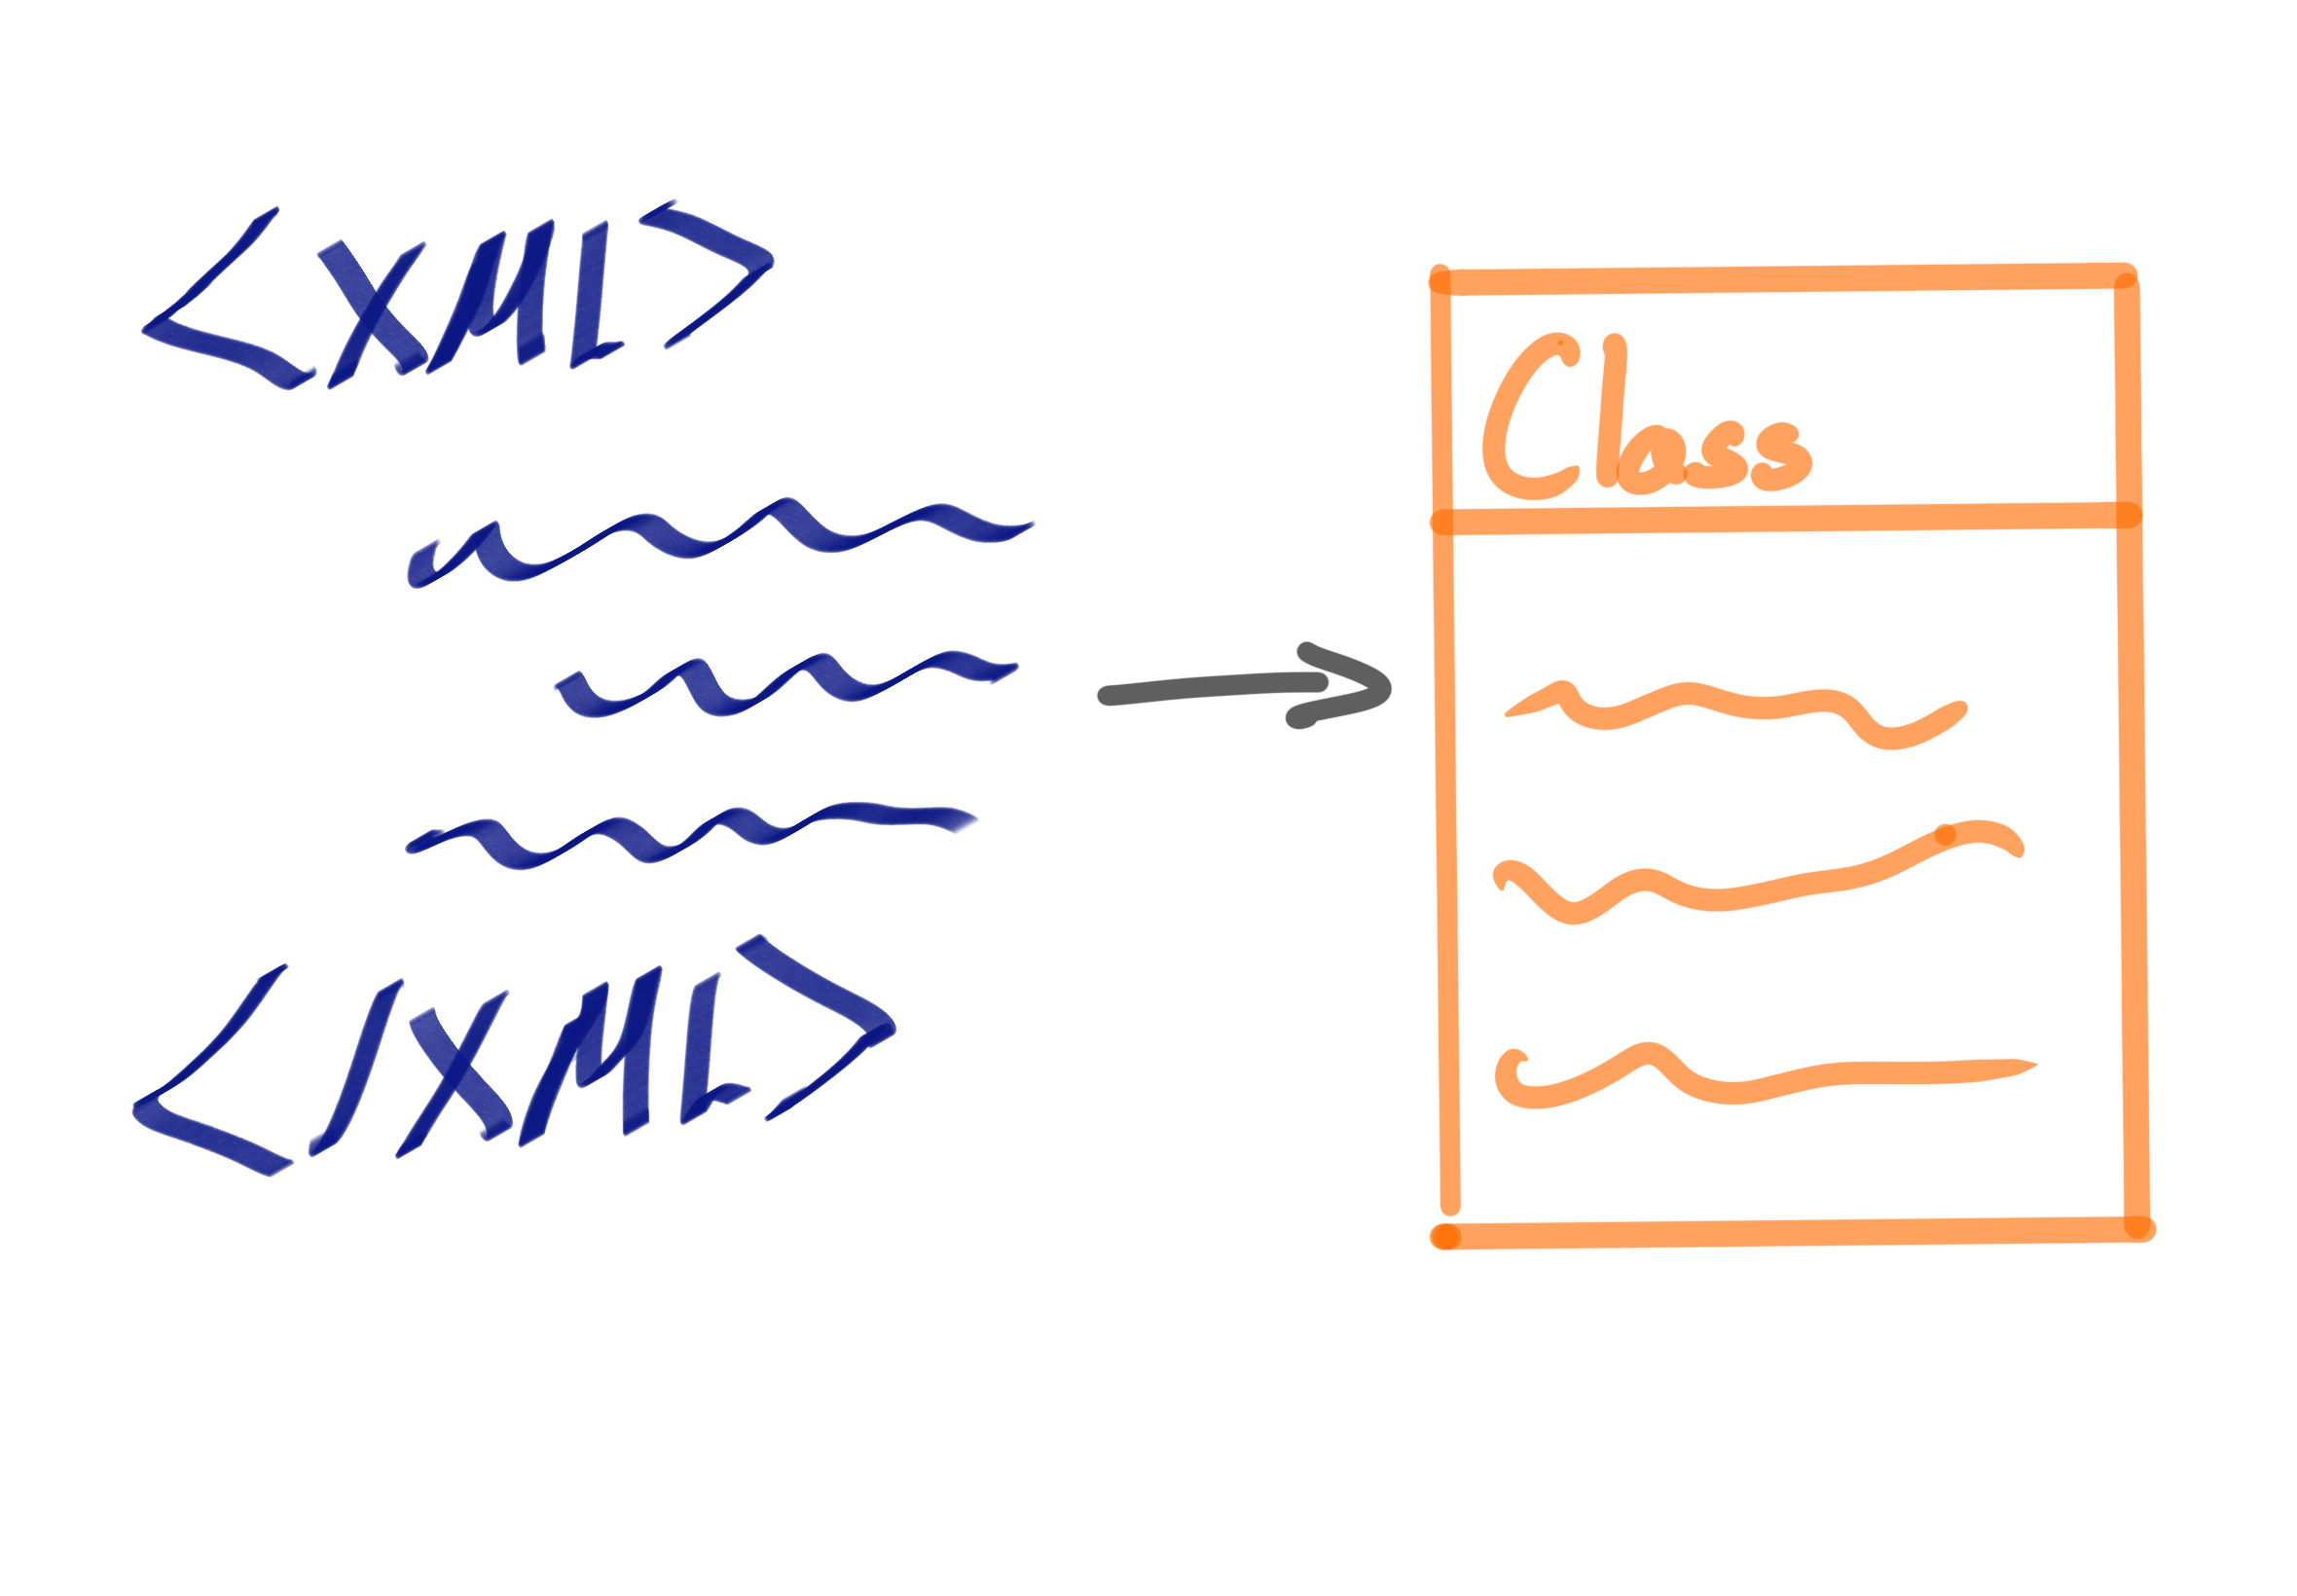
\includegraphics[width=0.6\textwidth]{images/xml.jpg}\\[1cm] 	% University logo
\vfill 
\end{titlepage}

\section{Objectives and Overview}

By the end of this assignment:
\begin{itemize}
  \item A review of constructing classes and instantiating objects in Java
  \item A review of overriding functions
  \item Reading XML files in Java.
  \item Using the parsed XML data to instantiate objects.
\end{itemize}

\section{Structures and Specifications}

This assignment will consist of the following files:
\begin{itemize}
  \item \lstinline|vehicles.xml| \textrightarrow\ A large XML file from the US Department of Energy containing data on vehicles.
  \item \lstinline|Vehicle.java| \textrightarrow \ The object we will use to store information on each vehicle from vehicles.xml.
  \item \lstinline|VehicleDatabase.java| \textrightarrow\ This class will be used to (1) parse in the file, (2) instantiate \lstinline|Vehicle| objects based on the XML elements that are parsed, and (3) allow the user to use query information in order to search for vehicles.
  \item \lstinline|VehicleInfoSearch.java| \textrightarrow\ Uses the \lstinline|VehicleDatabase| object to setup a small filter-based, search engine. 
\end{itemize}

In combination, these files will power an app that (1) reads in data from the
XML file, (2) cleans that data and constructs a List of objects from it, and
(3) returns filtered results based on a user query.


\subsection{vehicles.xml}\label{ref:xmlstuff}

The general format of the original file is quite verbose and contains more data
than we need. The process of extracting these fields will be detailed in the
next section but for now, here is the list of the ones you should be interested
in:
\begin{enumerate}
  \item \lstinline|<cylinders> INTEGER </cylinders>| \textrightarrow \ A count on the number of cylinders.
  \item \lstinline|<drive> STRING </drive>| \textrightarrow \ Indicates what type of drive the car is (e.g., rear wheel drive).
  \item \lstinline|<fuelType> STRING </fuelType>| \textrightarrow \ The type of fuel  the engine works on (e.g., Gas, Diesel).
  \item \lstinline|<make> STRING </make>| \textrightarrow \ The brand of vehicle.
  \item \lstinline|<model> STRING </model>| \textrightarrow \ The model of the vehicle.
  \item \lstinline|<year> INTEGER </year>| \textrightarrow \ The year of that make and model.
  \item \lstinline|<trans> STRING </trans>| \textrightarrow \ Indicates the transmission type.
  \item \lstinline|<VClass> STRING </VClass>| \textrightarrow \ The type of vehicle (e.g., truck, sedan).
\end{enumerate}

\newpage
\subsection{Vehicle.java}
To begin with, we will make a \lstinline|Vehicle| class which will contain
information on each of the vehicles we will eventually read in from our XML
file. 


\subsubsection{Attributes}
The first thing we will need for our class are some attributes to store
information on the vehicles that will eventually be instantiated. Reference
Section \ref{ref:xmlstuff} and create attributes for each of the vehicle
elements we will be storing information on. Be sure to (1) make each attribute
is of the correct type and (2) all attributes are \lstinline|private| and
\lstinline|final|. The purpose of \lstinline|private| is to ensure
encapsulation and \lstinline|final| is used to ensure that, once set, the
values associated with each attribute cannot be changed.\\

\subsubsection{Constructor}
Our constructor should have the following general form:
\begin{lstlisting}[frame=trBL]
public Vehicle(...){
    // Body here
}
\end{lstlisting}
\textbf{Your Task: } Complete the constructor such that it takes parameters for
each of the vehicles attributes and sets them. Refer to the attributes in section
2.2 for which attributes should be included in the constructor and what their
type should be.\\

\subsubsection{Getters}\label{sec:getter}

Since our attributes were declared with the \lstinline|private| keyword they
will not be accessible outside of the class. This keyword allows us to control
access to attributes by defining ``getter'' functions to allow instances of our
class, as they're used in other classes, access to private variables.
Additionally, we can allow other classes to modify the values of private
variables using ``setter'' functions.\\

For our Vehicle class we will only be needing to define getter functions since
all of our attributes are \lstinline|final| and therefore cannot be modified
after their initial assignment.  In general, getters function names should be
the word ``get'' followed by the name of the attribute we want to get. For
instance, if your class has a private attribute string attribute named
\lstinline|studentName| the associated getter function name should be:
\begin{lstlisting}[frame=trBL]
public String getStudentName(){ 
    return studentName;
}
\end{lstlisting}

\textbf{Your Task:} Define a getter for all of the attributes of your class
using this general form.\\


\textit{Hint: Defining getters and setters is tedious so most modern IDEs can
auto-generate getters and setter. Explore your IDE and see if you can figure
out how to use this functionality.}

\subsubsection{String Overrides}

Finally, we want the ability to print the contents of our class in a pretty,
readable manner. By default, if you instantiate a class and then print it 
you will get the something along the lines of the following output:\\
\vspace{0.2cm}\\

\begin{framed}
\begin{minipage}{0.25\textwidth}
\underline{\textbf{Foo.java}}
\begin{lstlisting}
public class Foo{
   //...
}
\end{lstlisting}
\end{minipage}
\hfill
\vline
\hfill
\begin{minipage}{0.32\textwidth}
\underline{\textbf{Main.java}}
\begin{lstlisting}
public class Main{
   Foo c1 = new Foo();
   System.out.println(c1);
}
\end{lstlisting}
\end{minipage}
\hfill
\vline
\hfill
\begin{minipage}{0.28\textwidth}
\underline{\textbf{Terminal:}}
\begin{shell}
> java Main
Foo@6504e3b2
\end{shell}
\end{minipage}
\end{framed}
\vspace{0.2cm}

By overriding the \lstinline|toString| function we can define how this class
should be converted to a string. This in turn defines what string should be
printed when printing an instance of the class. For instance, if the
\lstinline|Foo| class has an attribute \lstinline|name| we can provide a 
\lstinline|toString| method for that class and our program will now run
in the following way:\\
\vspace{0.2cm}\\

\begin{framed}
\begin{minipage}{0.52\textwidth}
\textbf{Foo.java}
\begin{lstlisting}
public class Foo{
    public String name = "bar";
    //...
    @Override 
    public String toString(){
        return "Foo name: " + this.name;
    }
}
\end{lstlisting}
\end{minipage}
\hfill
\vline
\hfill
\begin{minipage}{0.42\textwidth}
\underline{\textbf{Main.java}}
\begin{lstlisting}
public class Main{
    Foo c1 = new Foo();
    System.out.println(c1);
}
\end{lstlisting}
\hline
\vspace{0.2cm}
\underline{\textbf{Terminal:}}
\begin{shell}
> java Main
Foo name: bar
\end{shell}
\end{minipage}
\end{framed}
\vspace{0.2cm}


\textbf{Your Task: } Override the \lstinline|toString| method such that when an instance of the \lstinline|Vehicle| class is printed it appears in the following form:
\begin{shell}
--Year Make Model--
Cylinders: CylinderCount
Drive: DriveConfig
Fuel Type: FuelType 
Transmission: TransmissionType
Class: VehicleClass

\end{shell}

\subsubsection{Comparable Override}

In your provided starter files you will notice that the constructor is declared in the following way:
\begin{lstlisting}[frame=trBL]
public class Vehicle implements Comparable<Vehicle>{
    //...
}
\end{lstlisting}
\lstinline|Comparable| is an interface. We will cover interfaces in greater
detail later but, for the time being it is sufficient to know that an interface
is a construct in Java which contains function headers which have not
been implemented. For \lstinline|Comparable|, one of these functions is the
\lstinline|compareTo| method which is used by functions such as
\lstinline|Collections.sort|. In a later portion of the assignment we will be
sorting collections of \lstinline|Vehicle| instances and, as such, we must
implement the \lstinline|compareTo| method by returning a comparison between
attributes in the class for which the \lstinline|compareTo| method has already
been implemented (e.g., \lstinline|String|, \lstinline|Integer|). For example:
\begin{lstlisting}[frame=trBL]
public class Foo implements Comparable<Foo>{
    String name;
    public Foo(String name){
        this.name = name
    }
    @Override
    public int compareTo(Foo other) {
        return name.compareTo(other.name);
    }
}
\end{lstlisting}


\textbf{Your Task:} Change the class such that it implements \lstinline|Comparable<Vehicle>| and implement the method \lstinline|compareTo| method such that it compares vehicle objects based on their year.

\subsubsection{Vehicle Class - Checklist}
\begin{itemize}
    \item Class Attributes:
        \begin{todolist}
            \item All needed attributes are declared.
            \item Attributess are \lstinline|private|.
            \item Attributess are \lstinline|final|.
        \end{todolist}
    \item Getters
        \begin{todolist}
            \item A getter function exists for each attribute.
            \item All getters are of the form \lstinline|getAttributeName|.
        \end{todolist}
    \item Overrides
        \begin{todolist}
            \item The \lstinline|tosString| method is present and returns a string of the specified format.
            \item The \lstinline|compareTo| method is present and returns the comparision between the intance and a \lstinline|Vehicle| instance that is passed in as a parameter. The comparison should be based on year of the vehicles being compared.
        \end{todolist}
\end{itemize}




\newpage
\subsection{VehicleDatabase.java}
he XML document we are given contains many many fields with various
information on each type of vehicle. We want our parse to do the following:
\begin{enumerate}
  \item Parse the data in using the XML java DOM parser.
  \item Filter out the data we are interested in and retrieve the values.
  \item Instantiate Vehicle objects with those values.
\end{enumerate}


\subsubsection{Attributes}

For our class we will need two \lstinline|private| attributes:
\begin{enumerate}
    \item \lstinline|vehicleDatabase|  \textrightarrow \  An \lstinline|ArrayList| of \lstinline|Vehicle| instances. This will contain all of the vehicles in our database.
    \item \lstinline|makes| \textrightarrow \ An \lstinline|ArrayList| of strings. This will contain a list of all the unique makes in our database.
    \item \lstinline|models| \textrightarrow \ An \lstinline|ArrayList| of string. This will contain a list of all the unique models in our database.
\end{enumerate}

\textbf{Your Task: } Create these attributes according to their
specifications. DO NOT initialize them however. We will do that later in our
constructor.

\subsubsection{Constructor and XML Parsing}

For this portion of the assignment, create a constructor that takes a single
string, \lstinline|filepath|. This file path is intended to be either an
absolute or relative path to an XML file of the same form as vehicles.xml. The
purpose of our constructor is to parse this file and use it's contents to
populate our class's attributes.

The general template for parsing an XML file in Java using \lstinline|javax| is as 
follows:
\begin{lstlisting}{\scriptsize}

DocumentBuilderFactor dbf = DocumentBuilderFactory.newInstance();

DocumentBuilder db = null;
try{
    db = dbf.newDocumentBuilder();
} catch(ParserConfigurationException e{
    //...
}

File f = new File(filepath);

Document doc = null;
try{
    doc = db.parse(f);
} catch(SAXException | IOException e){
    //...
}
\end{lstlisting}

Following this set of operations you will be left with \lstinline|dbf|. From there
you should use the \lstinline|doc.getElementsByTagName(tag)| to:
\begin{enumerate}
    \item To get a \lstinline|NodeList| of each vehicle in the file and iterate over that list. For each item in that list:
    \begin{enumerate}
        \item Get the 
    \end{enumerate}
\end{enumerate}

\subsubsection{Getters}

\textbf{Your Task:} 
The only getter you will need for this class is for the \lstinline|makes|
attribute. We will be building other query function that will allow the user to
interact with the database. Be sure to create the getter in accordance with
the specifications detailed in Section \ref{sec:getter}.

\subsubsection{Query Functions}

To interact with the ``database'' we will be implementing the following functions 

\paragraph{\lstinline|public ArrayList<String> queryClasses(String
user_make)\{ ... \}|} This function should  search the database, and return a
\textit{sorted} ArrayList of string containing all the \textit{unique} vehicle
classes that are of the specified \lstinline|user_make|. Be sure to ignore the
case of the string \lstinline|user_make| when making comparisons.

\paragraph{\lstinline|public ArrayList<String> queryModels(String user_make,
String user_class)\{ ... \}|} This function should search the database and return a
\lstinline{sorted} ArrayList of strings containing all the \textit{unique}
vehicle models present in the database that have the specified
\lstinline|user_make| and \lstinline|user_model|. Be sure to ignore the case of
the parameters when making comparisons.

\paragraph{\lstinline|public ArrayList<Vehicle> queryVehicles(String
user_model)\{ ... \}|} Search the database and return an ArrayList of all the
\lstinline|Vehicle| instances in the database that match the model specified in
the parameter \lstinline|user_model|. Be sure to ignore the case of
\lstinline|user_model| when making comparisons.



\newpage
\subsection{VehicleInfoSearch.java}
This class will only have the \lstinline|main| method and will structure the
search functionality of the database. It should be implemented using the
following steps:
\begin{enumerate}
    \item Generate a database using the provided XML file.
    \item Present the user with the list of available makes, ask them which they want, and store that input.
    \item Use the make they selected to query which classes of vehicle are available with that make, present the result, then ask the user which they want.
    \item User the previous make and class results to query which models are available, present the results of that query, and ask the user which they would prefer.
    \item User the user input from the previous step to query the list of all those models, iterate over that list, and print each vehicle object to the user.
    \item Ask the user if they want to continue. If they type \lstinline|q| terminate the loop; otherwise, continue.
\end{enumerate}
Your output, once finished, should look something like this:

\begin{shell}
Generating database...
Makes: [AM General, ASC Incorporated, Acura, Alfa Romeo, American Motors Corporation, Aston Martin, Audi, ...]
Enter a make: Audi
Classes: [Compact Cars, Large Cars, Midsize Cars, Midsize Station Wagons, Midsize-Large Station Wagons, ...]
Enter a class: Midsize Cars
Models: [100, 100 quattro, 200, 200 quattro, 200 quattro 20v, 5000 CS Turbo, 5000 CS quattro, ...]
Enter a model: 100

RESULTS:
--1993 Audi 100--
Cyliners: 6
Drive: Front-Wheel Drive
Fuel Type: Premium
Transmission: Automatic 4-spd
Class :Midsize Cars

--1993 Audi 100--
Cyliners: 6
Drive: Front-Wheel Drive
Fuel Type: Premium
Transmission: Manual 5-spd
Class :Midsize Cars

--1994 Audi 100--
Cyliners: 6
Drive: Front-Wheel Drive
Fuel Type: Premium
Transmission: Automatic 4-spd
Class :Compact Cars
...
\end{shell}

Do note that the above example has replace some of the output for makes,
classes, and models with ellipses. This is only to shorted the example. Your
code should output each of the lists in their entirety.



%\newpage
%\section*{Rubric}

%\section*{Instructor Notes}

%In addition to the core technical topics being introduced in this assignment
%there are some meta points that relate to how you teach computer science topics
%that should be noted as well. To often in computer science courses there is an
%over focus on the technical

\end{document}
